\documentclass[a4paper,12pt]{extarticle}
\usepackage{geometry}
\usepackage[T1]{fontenc}
\usepackage[utf8]{inputenc}
\usepackage[english]{babel}
\usepackage{amsmath}
\usepackage{amsthm}
\usepackage{amssymb}
\usepackage{fancyhdr}
\usepackage{setspace}
\usepackage{graphicx}
\usepackage{colortbl}
\usepackage{tikz}
\usepackage{pgf}
\usepackage{subcaption}
\usepackage{listings}
\usepackage{indentfirst}
\usepackage[colorlinks,citecolor=blue,linkcolor=blue,bookmarks=false,hypertexnames=true, urlcolor=blue]{hyperref} 
\usepackage[noabbrev]{cleveref}
\usepackage{indentfirst}
\usepackage{mathtools}
\usepackage{booktabs}
\usepackage[flushleft]{threeparttable}
\usepackage{tablefootnote}
% \usepackage{refcheck}

\usepackage{chngcntr} % нумерация графиков и таблиц по секциям
\counterwithin{table}{section}
\counterwithin{figure}{section}
\DeclareMathOperator*{\argmin}{arg\,min} 
\graphicspath{{graphics/}}%путь к рисункам

\makeatletter
\renewcommand{\@biblabel}[1]{#1.} % Заменяем библиографию с квадратных скобок на точку:
\makeatother

\geometry{left=2.5cm}% левое поле
\geometry{right=1.5cm}% правое поле
\geometry{top=1.5cm}% верхнее поле
\geometry{bottom=1.5cm}% нижнее поле
\renewcommand{\baselinestretch}{1.2} % междустрочный интервал
\RequirePackage{float}                

\renewcommand{\theenumi}{\arabic{enumi}.}% Меняем везде перечисления на цифра.цифра
\renewcommand{\labelenumi}{\arabic{enumi}.}% Меняем везде перечисления на цифра.цифра
\renewcommand{\theenumii}{\arabic{enumii}.}% Меняем везде перечисления на цифра.цифра
\renewcommand{\labelenumii}{\arabic{enumi}.\arabic{enumii}.}% Меняем везде перечисления на цифра.цифра
\renewcommand{\theenumiii}{\arabic{enumiii}.}% Меняем везде перечисления на цифра.цифра
\renewcommand{\labelenumiii}{\arabic{enumi}.\arabic{enumii}.\arabic{enumiii}.}% Меняем везде перечисления на цифра.цифра

% \crefname{section}{глава}{глава }
% \Crefname{section}{Глава}{Глава }
\crefname{figure}{fig.}{fig. }
\Crefname{figure}{Fig.}{Fig. }
% \crefname{table}{табл.}{табл. }
% \Crefname{table}{Табл.}{Табл. }

\begin{document}

\section{Introduction to the problem}

Orienteering \cite{orienteering} is a sport that requires athletes to run with a map, following a certain cet of rules about the destination of the run.
In most cases, they shall run through specified locations in specified order as fast as possible.
Orienteering can be done in cities, forests, mountains, malls, and so on.

The only thing that athlete has left after the race is the map, and for professional athletes it is crucial to do post-analysis of their race performance.
For some races, such as city races, route choice problem is the main subject of such analysis.
And it is important to find all routes available and compare their length, which might be hard without an analyzer tool.

\subsection{Problem statement}

This project aims to create a tool that will do analysis of routes for orienteering city races.
Our tool allows to find the optimal route for each control of an orienteering course, but we also propose a theoretical
algorithm to find multiple different optimal paths as well.

\subsection{Related applications and technologies}

\begin{enumerate}
    \item Livelox \cite{livelox} is a website created for orienteering competitions, where jury can upload map with distance configuration, and athletes can upload their GPS tracks.
The data used by organisers is private. 
    \item The maps and courses are usually created with specific software such as OCAD \cite{ocad} and openorienteering \cite{openorienteering}. 
Such software creates data files that have precise vectorized description of a map, but these files are mostly private, and community only has a jpeg version of a map.
    \item Tools, similar to our project, are used for world cup translations \cite{worldcup}, but they are propriate and use private data as well.
\end{enumerate}

All these tools do not have a built-in solution for route analysis, and most of them require specific data which is not available for athletes.

\section{Implemented methods}

We created a pipeline consisting of several algorithms that decomposed the problem and provided step by step solution with the ability to change the implementation of any block in case results are not good enough.
Because of the fact that one stage might heavily depend on previous one, we decided that it is necessary to allow manual modification of intermediate data.
Otherwise the prediction errors will be stacked together.


Overall, the developed pipeline is the following:
\begin{enumerate}
\item Extraction of circuit (\textit{course, race configuration}) layer with U-Net model \cite{unet}
\item Extraction of obstacles (\textit{lakes, buildings, fences, etc}) with U-Net model \cite{unet}
\item Detection of circles based on modification of Hough circles transform \cite{houghcircles} and special kernel 
\item Detection of triangles based on OpenCV contour detection \cite{findcontours}
\item Extraction of information about the course configuration with TSP solver \cite{tspsolver} on course layer with special scoring matrix
\item Selection of the best routes for each control with $A^*$ algorithm \cite{astar}.
\end{enumerate}


\subsection{Semantic segmentation for layers separation}

For first two steps of pipeline we had to separate layers of map data from the image.
The image itself is a simple scheme with all kinds of shapes and colors, where all signs are standartized by International Orienteering Federation \cite{iof}.
The problem with the data is the fact that objects are not real-life objects, so pretrained computer vision models are not useful for us.
Overall, the structure of image is based on some set of rules, that are hard to express in a formal way.
These rules are hard to learn artificially, because there are same colors used for different types of things, and objects are not consistent in terms of forms and shapes.
Also, there are connections between objects, that are really hard to find in general case (\cref{mapsample}).

We decided that the best approach we have is to solve a semantic segmentation problem.
Indeed, label of a pixel is mostly based on its color, generic form of shape it belongs to, and surrounding objects, so the detection problem is local and can be solved using $128 \times 128$ patches of a map.

There are no labelled public datasets of orienteering city maps, so we found some open archives of orienteering maps and selected a sample of 50 maps by hand.
To label this data for semantic segmentation problem, we used a special python package labelme \cite{labelme}, that allows to manually select shapes on top of the image given.
We initially labelled 27 images for segmentation of runnable layers. One day prior to deadline we also have labelled 12 full courses.

Labelme produces json array with description of all the shapes (we used lines, circles, and polygons).
To create a mask out of the json description of a shape border, following algorithm was used:
\begin{enumerate}
    \item Take shapes one by one and determine its bounding box.
    \item For every pixel in bounding box, check if pixel belongs to a shape.
    \item To finding if the point is inside the shape, point-to-segment distance was used for lines, circle equation was used for circles and well-known algorithm for polygons \cite{pipproblem} that casts the ray from the point and checks if number of intersections with edges is odd.
\end{enumerate}

As a baseline, we had a set of rules based on HSV color space.
It allowed us to capture <<red>> layer which is mostly used for circuit, <<olive layer>> that represents prohibited area, <<blue layer>> that represents water.
But it doesn't take overlaps into account and confuses different objects if they share a color.

\subsubsection{CNN for detecting circuit layer}
\subparagraph{Motivation for the model\\}

To try and outperform the naive implementation, we developed and trained a CNN \cite{cnn} to detect the circuit layer, e.g the layers that notated where the start/end points of a track lied, the connections between tracks, and the labels for each track.
The motivation for creating this CNN was that we could not be sure that a naive implementation of removing layers based on color alone would work well, and we hoped that a simple CNN could detect connected circles, triangles, and lines of the same color and thickness in order to remove them from the final map. 

\subparagraph{Creating training and validation sets with masks\\}

In order to train the CNN with a limited data-set, we took maps without circuits, in other words maps that were ready for path detection, and added layers on top of them so that we could have ample training and validation sets. This included drawing a random number of circles, lines, and text using cv2 functions, ensuring that the locations of the circles were spread out and the lines connected the circles, and using a variety of colors (though uniform per training image). All in all it was fairly simple and allowed us to produce however many training/validation images as we wanted. To produce the masks for the training and validation sets, all that needed to be done was feed in the color that was used to create the figures on the training/validation images into a function that took a “bitwise and” of the image and a mask of that color. Then just converting the mask to black and white produced good results.

\subparagraph{Creating the CNN model\\}
We created a simple CNN model (\cref{fig:simple-CNN}) with 2 convolution layers and no pooling layers, figuring that all the CNN would really do is learn the intended colors to remove, since the figures to be removed were uniformly colored. The model would take in a colored 200x200 random segment of each colored image, and output a black/white mask as intended. For the model we experimented with different loss functions, and decided on Binary Cross Entropy loss, which is used commonly for binary classification tasks. For the optimizer, we learned that the Adam optimizer produced results similar to though more effective than Stochastic Gradient Descent, and ran with that.



\subparagraph{Problems with the model\\}
Eventually we realized that for the task of circle detection we needed the model to do more than just separate the layers based on color.
There were often parts of the map that were the same color as the layers we intended to remove, and we didn't want to segment them in the layer detection model.
This was because the circle detection was much less effective if there were layers interrupting the circles. So we attempted to reconfigure the model to ideally just identify the circles and lines, ignoring other figures like labels of the circles and other figures in the map (areas that were out of bounds often were colored the same as the circles/lines).
Our reasoning for the current state of the model was that it should have already been able to do more than simple color identification, if we just modified the training masks to only include the lines and circles. We did this and also attempted to incorporate max pooling which should have made line detection easier \cite{cnnsemanticsegmentation}. Unfortunately this model (\cref{fig:pooling-CNN}) did not produce adequate results, and we were ultimately unable to use it.


\subparagraph{Training the model\\}
Using the images and masks that we had created, we made tensors which could be fed into pyTorch data loaders \cite{pytorch}.
This involved creating random crops of the masks and images. One problem we had to overcome, which turned out to be relatively simple, was ensuring that the random crops were of the same section for the images and corresponding masks. With our training and validation data loaders, we were able to train the model in the corresponding fashion (\cref{fig:training-loop}). With our model fully trained, we were able to test it on a testing set that was filled with maps with layers on top. While it did produce great results on maps where the layers to be removed were the only ones of that color, since the model was essentially just detecting the colors of the layers it produced a decent amount of noise on non-ideal maps. Before attempting to modify the model to only separate circles/lines, we thought that we would be able to remove the noise in order to isolate the intended figures for the later circle detection algorithm. However, as we discovered the main problem was not removing noise, which did not really hinder the way we detected the circles, but rather the presence of larger figures like pink areas on the map or the numerical labels of the circles. 

\subsubsection{U-Net for detecting obstacle layer}

For detection of a runnable layer, we also tried CNN model.
The problem with results was the same: if model doesn't use pooling, it can't extract enough information from surrounding context and is solely based on a color of a pixel.
If it has pooling, than it has hard time recovering label for specific pixel during upsample stage.

Then we tried U-Net \cite{unet}. Advantage of the U-Net is its ability to have a context of real pixel values and look at the high-level descriptors as well.
So we created a compact version of U-Net that takes 10 minutes to train, weights less than a megabyte and works relatively well.

The implementation is based on keras with tensorflow \cite{keras}, we also used albumentations \cite{albumentations} package to augment the dataset.

\subsubsection{U-Net for detecting circuit layer}

When we finished all other parts of pipeline, we tried to apply the same U-Net approach to circuit layer detection.
We labelled a small dataset of maps and trained U-Net.
Initially, it struggled to extrapolate its knowledge, and while it produced great results on training set, test results were just a noise.
After experiments we found out that it relied on the image dimension. So we used maxpooling to downsample high-resolution image.
Also it had a hard time understanding different colormaps so we retrained it on the output of our baseline model, that basically produces <<the red layer>>. 

Suprisingly, after these two changes results became great (\cref{unetcircuitresult})

\subsection{Detection of course configuration}

Course configuration consists of triangle, which is a start, set of circles, that represent controls, and lines that are used for connection (\cref{examplecircuit}).
In general, there are many possibilities for race rules, that may result in map having several start points, more than two connections for a control or even no connections at all.
We decomposed our detection process the way that shapes detection is separated from connecting objects so intermediate data might still be useful.
Consiedring connections between controls, there are many challenges and modes to consider for every single race type.
So, for the sake of simplicity, we limited out problem to courses when  configuration is a permutation of circles, which is the most common one.

\subsubsection{Algorithm for triangle detecction}

To find a start is a problem of finding a triangle.
We know that the given triangle is going to be equilateral.
To find it, we need to address the challenge of a noise in the data.
In general, openCV provides a way to find a custom polygon \cite{findcontours}
The problem with the method is that it expects polygon to be filled, when triangle from our dataset only has contours.
Not only the triangle has contours, but it also has adjacent line, so using default algorithm is not an option.
Our algorithm uses dilation and erosion to remove noise around the triangle and keep only the pixels inside of a contour:
\begin{enumerate}
    \item Image is dilated by $d$ pixels, where $d$ is a hyperparameter that equals $0.3-0.5$ of expected triangle size.
    \item After the dilation, triangle becomes solid, and all adjacent lines are not wider than $w + 2 * d$, where $w$ is an initial width of lines
    \item At the same time, the contour of triangle already has $d + w$ outside pixels. Now we do erosion for $e$ pixels and delete the lines and noise, keeping the inside of the triangle untouched for openCV detector. $e \approx d + \frac{w}{2} + \epsilon$
    \item Now we select polygons using openCV detector and filter those that are equilateral triangles.
\end{enumerate}

The issue we found with the algorithm is that it is dependent on two hyperparameters $d$ and $e$.

\subsubsection{Algorithm for circle detection}

To find circles, Hough circles method was used as the first approach \cite{houghcircles}.
The problem with this method is that it detects all circles, not only ones with fixed radius.
Also during our experiments we found it hard to tune its hyperparameters and algorithm provides a lot of false positives that need to be filtered out, so the overall pipeline is messy and does not generalize well.
As with triangles, additional challenge was that circles are corrupted and they have adjacent lines as well.

Our algorithm works as following:
\begin{enumerate}
    \item For every pixel that is labelled as a part of circuit layer, we add $+1$ to all pixels that are distance $r$ away from it.
    \item Then we select pixels that have an accumulated sum bigger than $candidate\_threshold$. It means this pixel has a lot of information in its r-neibourhood and we need to check it.
    \item For every candidate circle center we take $2r \times 2r$ region and try to understand if it is a circle or not. it might be a solid surface, corner of rectangle or something else. To do so, we create a special $2r \times 2r$ kernel \cref{fig:circlekernel}, that has a lot of 1's on the circle border and a lot of -1's near the center.
    \item When we take a sum of pointwise multiplications we get a total $score = border\_pixels - inside\_pixels$, because of the kernel structure.
    \item We concider circle present in the layer if $score > match\_threshold$.
    \item If circle has a high score, we filter out all the circles in its $r$-neighborhood, so we dont face problem with duplications. 
\end{enumerate}

Our algorithm has 3 hyperparameters: $r$, $candidate\_threshold$, $match\_threshol$.

\subsubsection{Algorithm for configuration detection}

Because we know that configuration is a permutation. all we have to do is to find a permutation of points (control points + start), where each pair of adjacent points is connected in the course layer.
Lines can intesect, they can miss some segments, they might not even be straight, so there is no way to find the exact permutation.

So, to find a permutation, we construct a pairwise scoring, which shows how close the points are.
Then we can use pairwise scoring as a graph representation and solve TSP problem \cite{tsp} with annealing-based TSP-solver \cite{tspsolver}.

Scoring takes two things into account:
\begin{enumerate}
    \item Most of the connections are straight lines.
    \item Some connections are not.
\end{enumerate}

We found out that it is helpful to create two scores $score_{line}$ and $score_{distance}$ and use their combination to take both cases into account:
$$score = \min(score_{line}, 2 \cdot score_{distance})$$

For $score_{line}$, we take all the pixels on the line between two points and calculate the share of pixels that aren't present in the line $l$:

$$score_{line} = \frac{|p = 0, p \in l|}{|l|}$$

For $score_{distance}$ we assume that connection is not a straight line (or it misses some pixels inside) and we need to find a path that is most likely to be a drawn connection between two points.
For that, we create a graph, where going through a pixel on the circuit layer is 10 times shorter then going trough a pixel outside of it.
Then we find a shortest path using $A^*$ \cite{astar}, that would try its best to use circuit layer where possible because of the graph structure.

After we initially developed this algorithm, we faced the fact it is extremely slow when it needs to find pairwise score for 20-30 circles.
To address this issue, we compressed the graph: we've built quadtree \cite{quadtree} on top of the circuit layer, where a node becomes a leaf, if all underlying region has the same pixel type.
Because of this structure, we compress big parts of a map, that have no useful information.
It made the scoring algorithm approximately 40 times faster for our use case.

\subsection{Shortest path analysis}

Having obstacles labelled, we just had to run $A^*$ algorithm \cite{astar} on a pixel grid with euclidean distance, where pixels, that are labelled as obstacles, are forbidden to go through.

\section{Result: a Streamlit-based web application}

There are many steps of the pipeline where something can go wrong, so as we were doing proof-of-concept application, we made a web application that allowed us to modify hyperparameters interactively and correct output of detectors if they are mistaken.
We use sliders and text inputs instead of draggable web components that could be done by skilled web developer and Javascript guru.
Creation of a good web interface is an important and challenging task to do in the future, but it is not related to the content of INF-573.

Application was built on top of Streamlit \cite{streamlit} framework which allows to use Python for creating simple interactive websites with the help of mpld3 \cite{mpld3} library, that allowed to draw matplotlib figures on the website.

\section{Extra: ideas for the future}

First of all, we have a full hypothesis on generated data for model training, that we tested poorly.
We are sure it is possible to train U-Net on a combination of artificial dataset and real data to get even better results.

Another problem is that our algorithm is unable to show several best routes that aren’t <<equivalent>>.
We managed to understand a problem and thought of a way to solve it, but it is a challenging task that would require twice as much time as everything we've done before:
\begin{enumerate}
    \item Two routes are equivalent if they can be continuously modified so one turns into another without crossing the obstacles.
    \item It is possible to build Voronoi diagram-like structure \cite{voronoipolygon}, separating each pixel based on the closest obstacle.
    \item It would mean that every pixel is now between two obstacles and each path can be classified by sequence of regions.
    \item Then it would be possible to compress each region into a single vertex and find several shortest paths on a compressed graph.
\end{enumerate}

We are leaving this task to future ourselves or those who will continue our work.





% \nocite{*}

\newpage
\section{Appendix}

\begin{figure}[H]
    \centering
    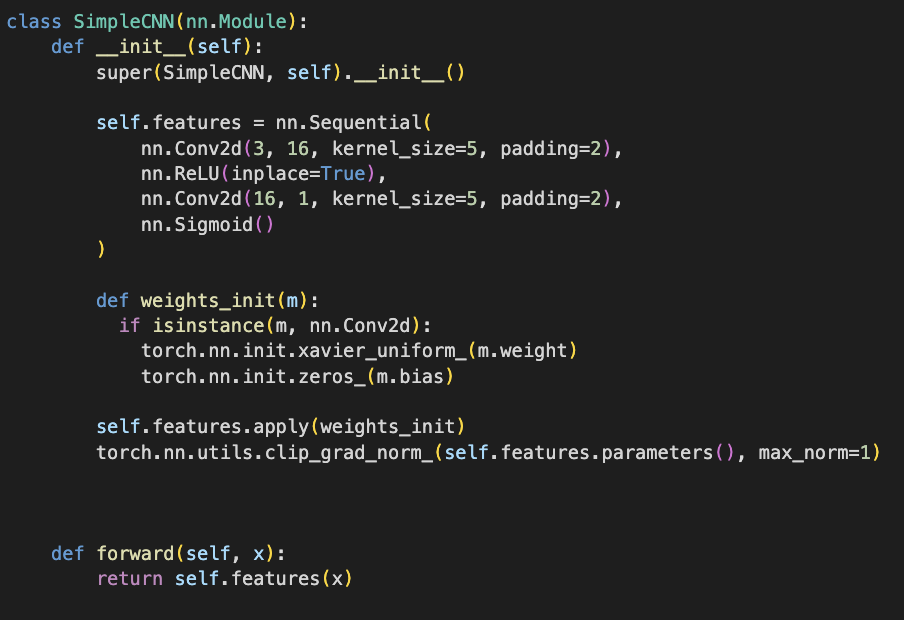
\includegraphics[width=\linewidth]{CNN simple model.png}
    \captionof{figure}{Simple CNN Model}
    \label{fig:simple-CNN}
\end{figure}
\begin{figure}[H]
    \centering
    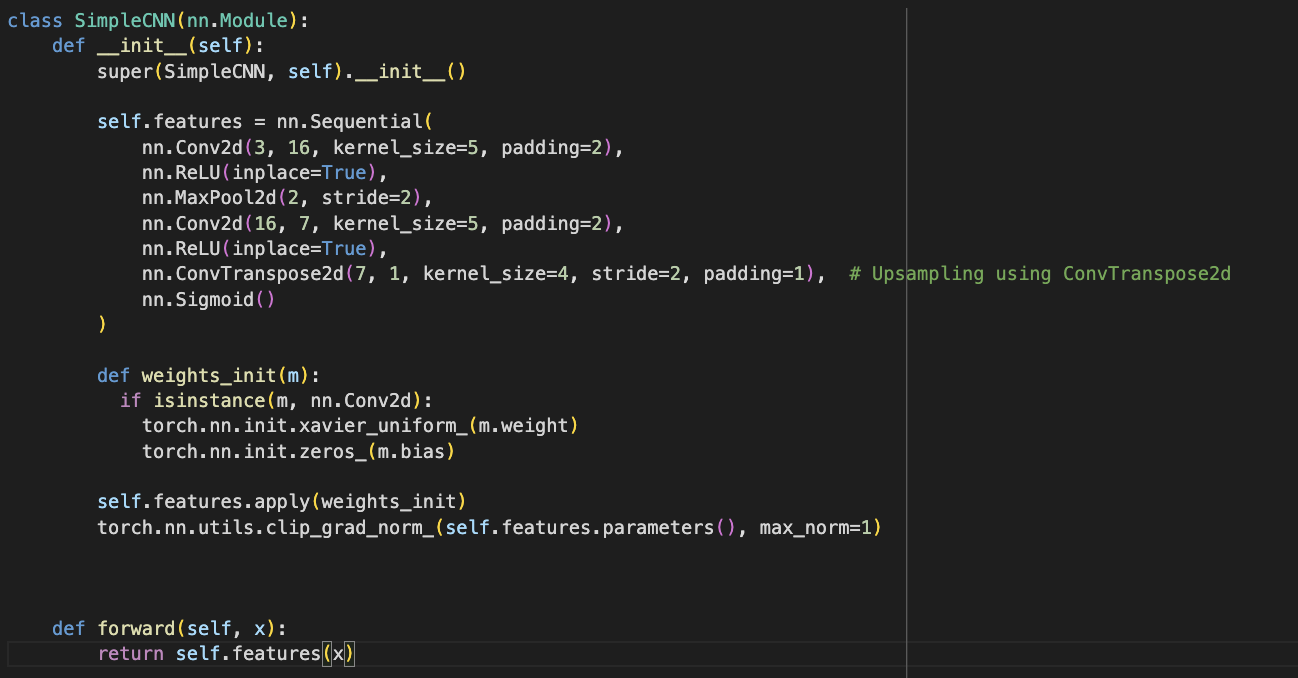
\includegraphics[width=\linewidth]{CNN model pooling.png}
    \captionof{figure}{Attempted CNN Model with pooling}
    \label{fig:pooling-CNN}
\end{figure}
\begin{figure}[H]
    \centering
    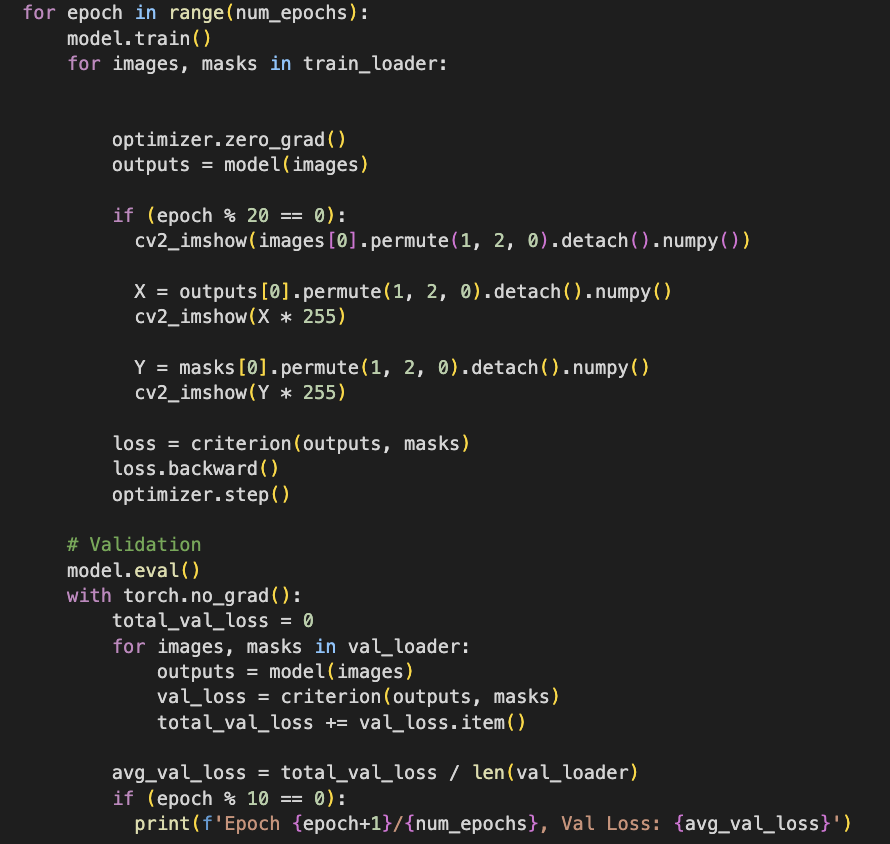
\includegraphics[width=\linewidth]{CNN training loop.png}
    \captionof{figure}{Model Training Loop}
    \label{fig:training-CNN}
\end{figure}
\begin{figure}[H]
    \centering
    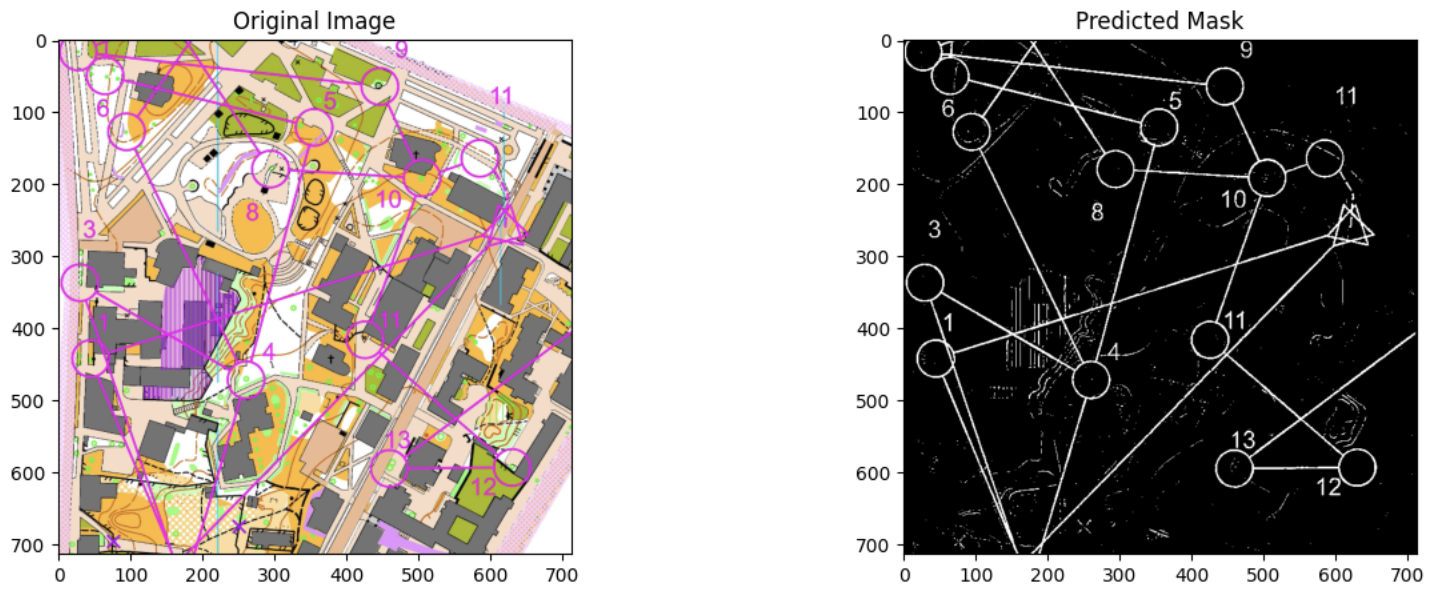
\includegraphics[width=\linewidth]{Predicted mask.png}
    \captionof{figure}{Original Image and Predicted Mask}
    \label{fig:prediction-CNN}
\end{figure}
\begin{figure}[H]
    \centering
    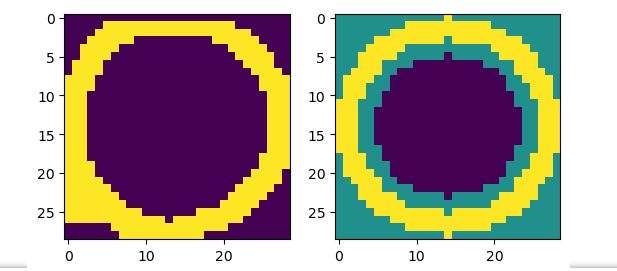
\includegraphics[width=\linewidth]{circle_kernel.png}
    \captionof{figure}{Patch for circle detection and circle kernel.}
    \label{fig:circlekernel}
\end{figure}


\newpage
\begin{thebibliography}{00}
\bibitem{orienteering} Orienteering, Wikipedia --- URL: https://en.wikipedia.org/wiki/Orienteering 
\bibitem{livelox} Livelox website --- URL: https://www.livelox.com/
\bibitem{openorienteering} Openorienteering Mapper application, --- URL: https://www.openorienteering.org/apps/mapper/ 
\bibitem{ocad} OCAD website, OCAD Inc, --- URL: https://www.ocad.com/en/ 
\bibitem{worldcup} Orienteering World Cup Round 1 2022, YouTube, --- URL: https://youtu.be/vwzoxJ2Bc0k?si=33TMbI07Ehfh\_jmc\&t\=308
\bibitem{unet} Ronneberger, O., Fischer, P., Brox, T.: U-net: Convolutional networks for biomedical image segmentation. In: MICCAI. pp. 234–241. Springer (2015) 
\bibitem{houghcircles} Hassanein, A. S., Mohammad, S., Sameer, M., \& Ragab, M. E. (2015). A survey on Hough transform, theory, techniques and applications. arXiv preprint arXiv:1502.02160.
\bibitem{findcontours} Satoshi Suzuki and others. Topological structural analysis of digitized binary images by border following. Computer Vision, Graphics, and Image Processing, 30(1):32–46, 1985. 
\bibitem{tspsolver} Fillipe Goulart, python-tsp, GitHub --- URL: https://github.com/fillipe-gsm/python-tsp
\bibitem{astar} Russell, Stuart J. (2018). Artificial intelligence a modern approach. Norvig, Peter (4th ed.). Boston: Pearson. ISBN 978-0134610993. OCLC 1021874142.
\bibitem{iof} IOF mapping specification, --- URL: https://orienteering.sport/iof/mapping/
\bibitem{labelme} Labelme, Kentaro Wada, GitHub --- URL: https://github.com/wkentaro/labelme 
\bibitem{pipproblem} Shimrat, M. (1962). Algorithm 112: position of point relative to polygon. Communications of the ACM, 5(8), 434.
\bibitem{cnn} Krizhevsky, A., Sutskever, I., \& Hinton, G. E. (2012). ImageNet Classification with Deep Convolutional Neural Networks. In F. Pereira, C. J. Burges, L. Bottou, \& K. Q. Weinberger (Eds.)
\bibitem{pytorch} Pytorch, https://pytorch.org/
\bibitem{cnnsemanticsegmentation} Le, James. “Semantic Segmentation Using Deep Learning.” Nanonets Intelligent Automation, and Business Process AI Blog, Nanonets Intelligent Automation, and Business Process AI Blog, 13 June 2022, nanonets.com/blog/how-to-do-semantic-segmentation-using-deep-learning/.
\bibitem{keras} Keras, https://keras.io/
\bibitem{albumentations} Buslaev, A., Iglovikov, V. I., Khvedchenya, E., Parinov, A., Druzhinin, M., \& Kalinin, A. A. (2020). Albumentations: fast and flexible image augmentations. Information, 11(2), 125. 
\bibitem{tsp} Goyal, S. (2010, April). A survey on travelling salesman problem. In Midwest instruction and computing symposium (pp. 1-9).
\bibitem{quadtree} Andrea Serreli, Pathfinding with Quadtrees and A*, --- URL: https://www.andreaserreli.me/post/pathfinding-with-quadtrees-and-a
\bibitem{streamlit} Streamlit, --- URL: https://streamlit.io/
\bibitem{mpld3} mpld3: A D3 Viewer for Matplotlib --- URL: https://mpld3.github.io/

\bibitem{voronoipolygon} Xiaolong Liu, \& Meixiu Yu. (2020, July 26). longavailable/voronoi-diagram-for-polygons. Zenodo. http://doi.org/10.5281/zenodo.3960407

\end{thebibliography}
	


\end{document}
